
\documentclass{article}
\usepackage{listings}
\usepackage[utf8]{inputenc}
\usepackage{graphicx}
\usepackage{subfiles}
\usepackage{wrapfig}
\usepackage{geometry}
\usepackage[italian]{babel}
\usepackage[export]{adjustbox}
\usepackage[font=scriptsize]{caption}
\usepackage{titlesec}

\titlespacing*{\section}
{0pt}{3ex plus 1ex minus .2ex}{3ex plus .2ex}
\titlespacing*{\subsection}
{0pt}{3ex plus 1ex minus .2ex}{3ex plus .2ex}
\graphicspath{ {./images/} }
\geometry{a4paper, top=2cm, bottom=2cm, left=2cm, right=2cm, heightrounded, bindingoffset=5mm}
\hyphenation{duplicate ip address}

\title{\Huge LABORATORIO DI INTERNET 
    \\ Report 1: Advanced Ping}
\author{Gruppo 21}
\date{Marzo 2021}


\begin{document}
\lstloadlanguages{C}

\maketitle

\begin{center}
    
\includegraphics[scale=0.75]{logo_poli.png}

    \vspace{20mm}

    Diego Zanfardino s256536, \\
    Fabio Trovero s258574, \\
    Lorenzo Ferro s260878

    \vspace{10mm}
    prof. Mellia Marco
\end{center}

\pagebreak

\begin{figure}
    \centering
    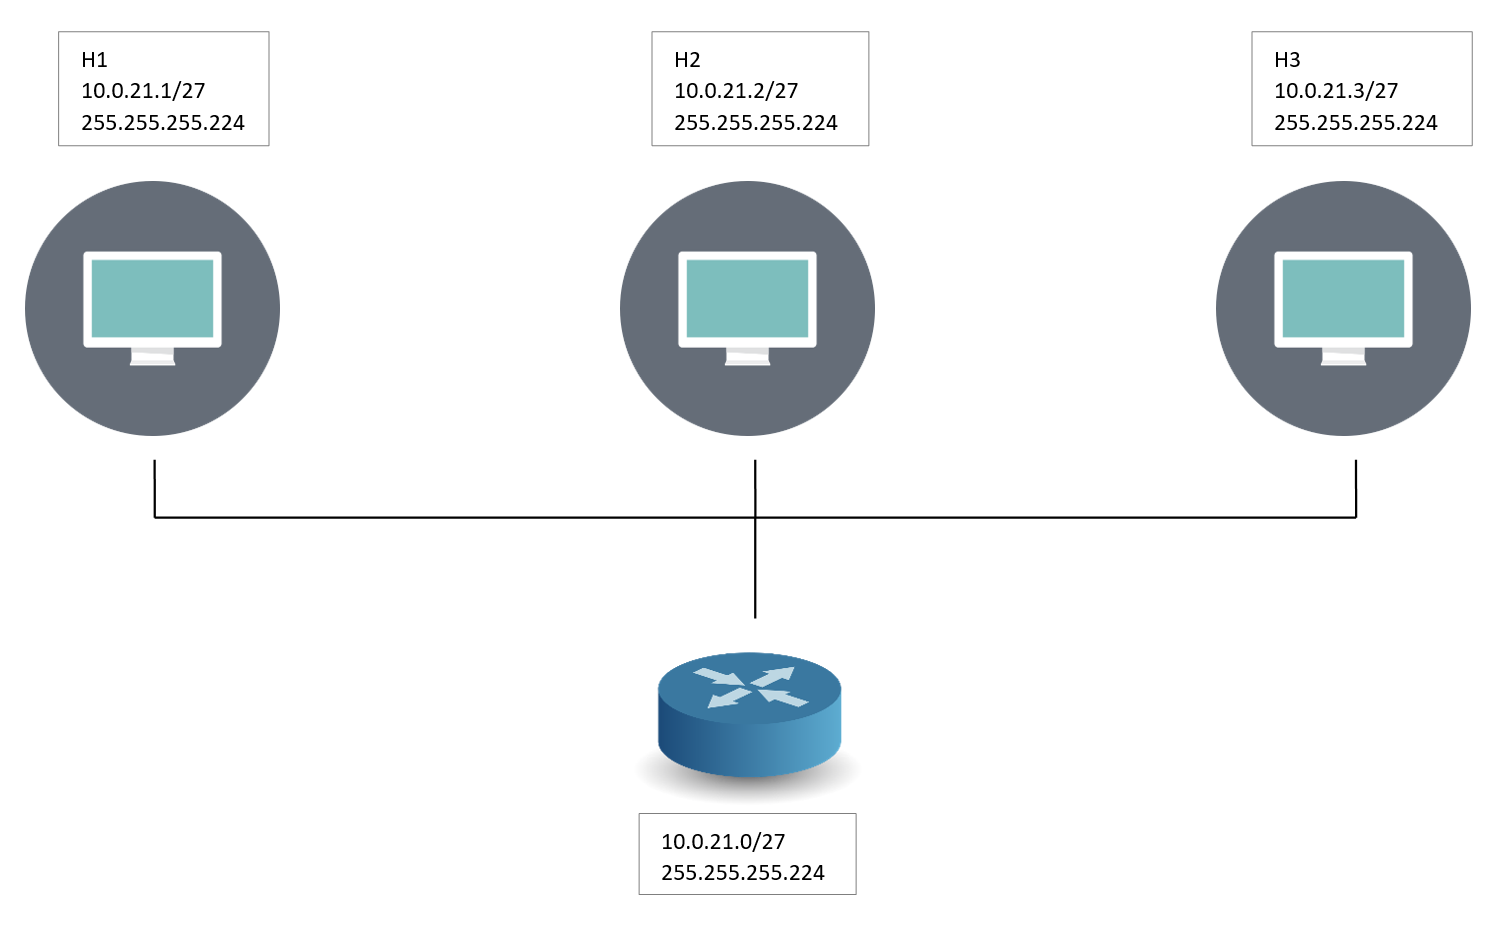
\includegraphics[scale=0.25]{rete1.png}
    \caption{Configurazione iniziale della rete}\label{Fig:data1}
\end{figure}

\section{Ping a indirizzo broadcast}
Per abilitare la risposta degli host ai ping verso gli indirizzi di broadcast abbiamo dovuto eseguire il seguente comando: 
$$sysctl net.ipv4.icmp\_echo\_ignore\_broadcasts=0.$$

\begin{flushleft}
  Eseguiamo il comando: ping 10.0.21.31 -b, aggiungendo l’opzione -b per permettere il ping al broadcast.
\end{flushleft}

%\hspace{1.2cm}
\begin{wrapfigure}{r}{0.5\textwidth} %this figure will be at the right
    \centering
    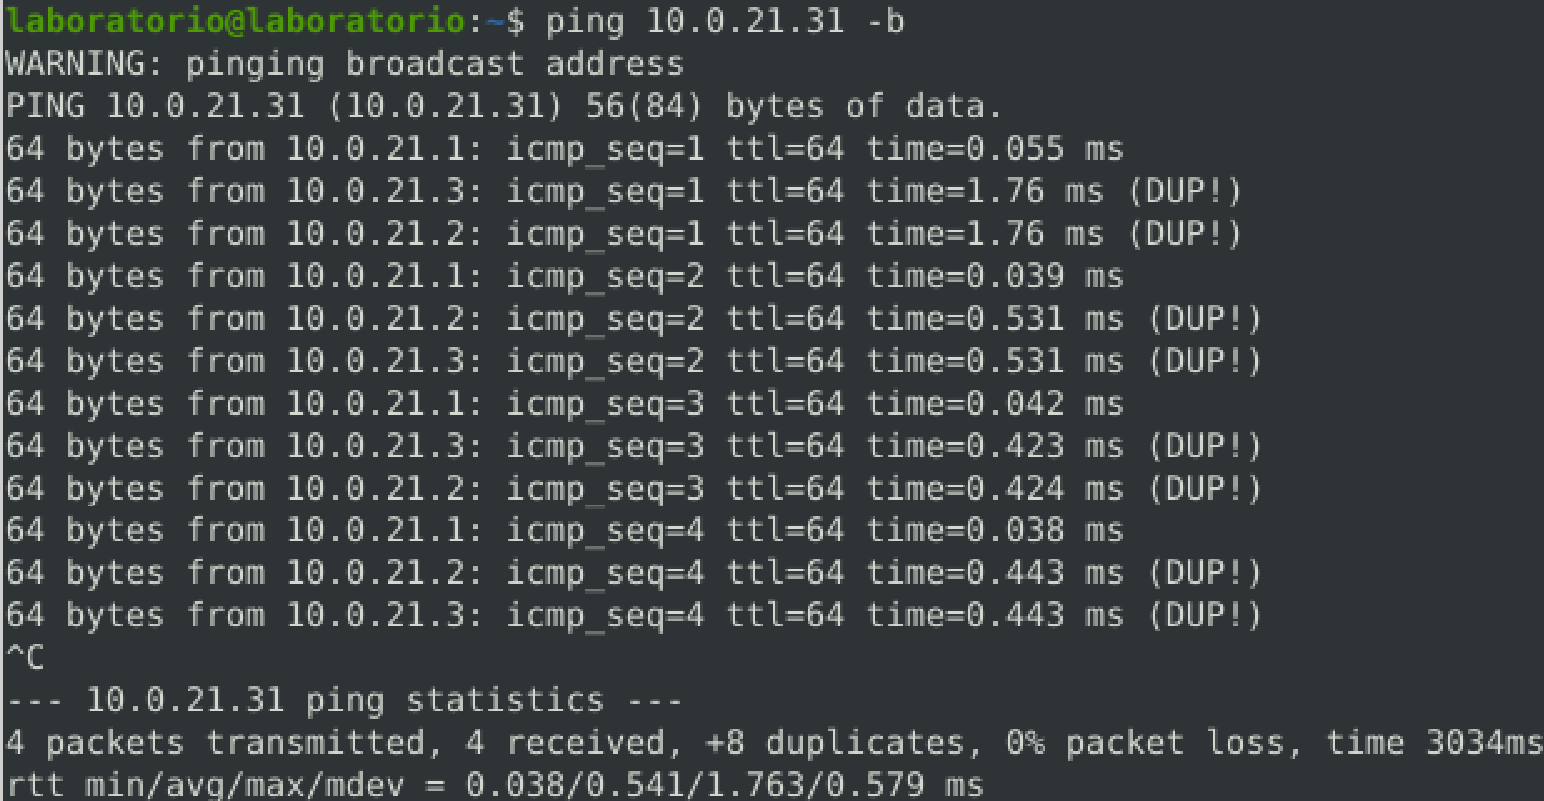
\includegraphics[width=0.5\textwidth]{broadcast1.png}
    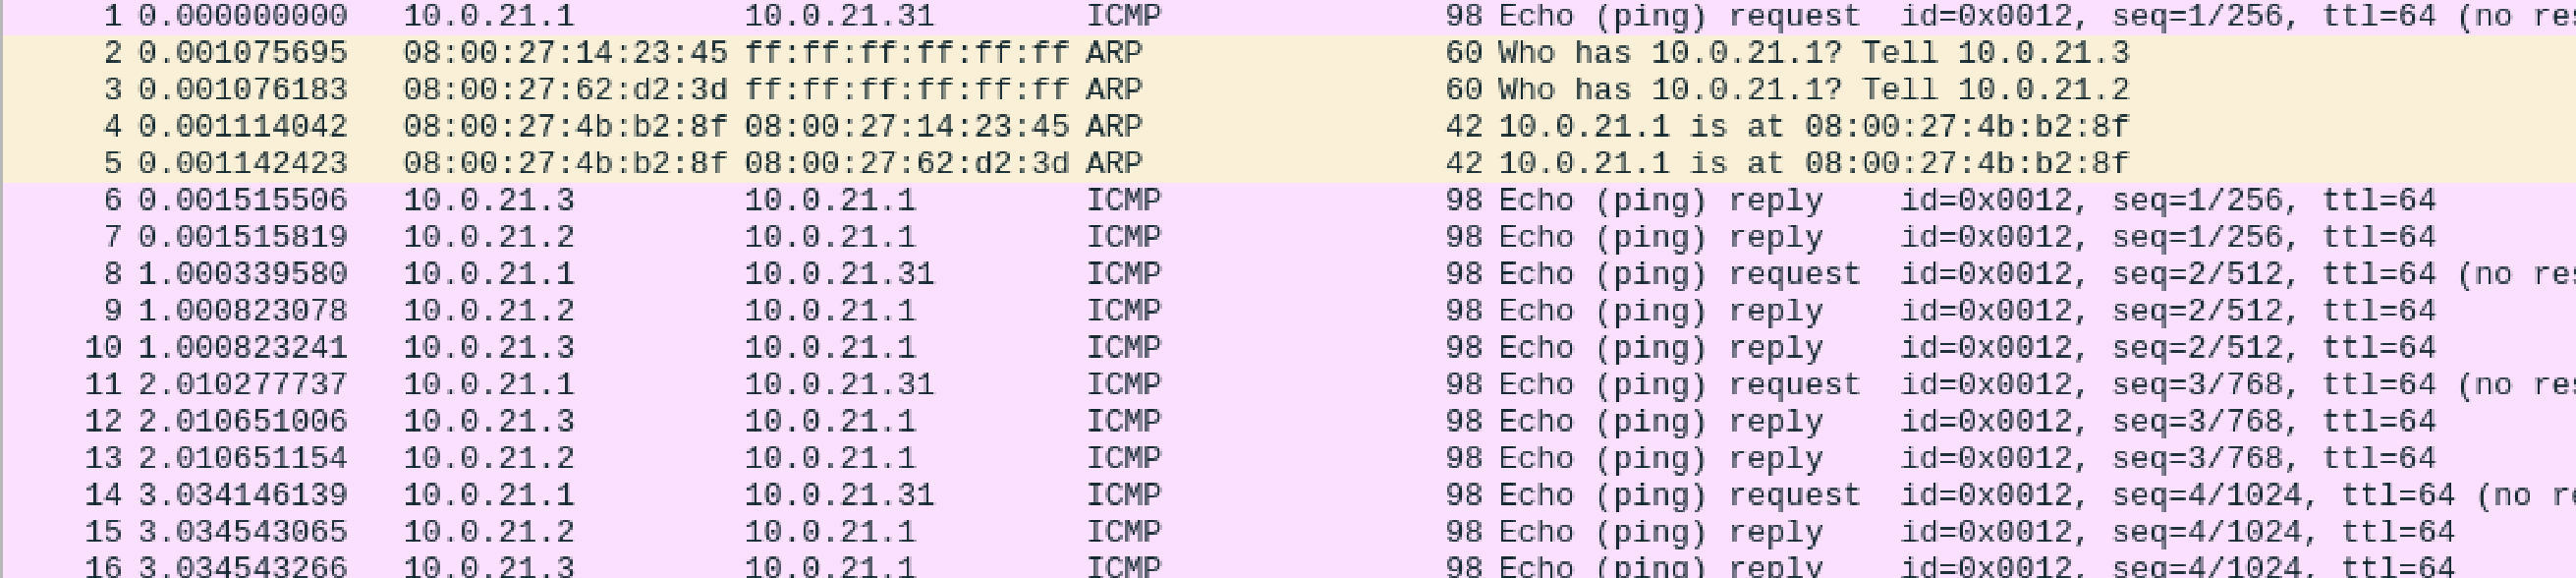
\includegraphics[width=0.5\textwidth]{wiresharkbroadcast.png}
\end{wrapfigure}

Si può notare che: \\
La prima risposta ricevuta è quella dell’interfaccia di loopback dell’host che effettua il ping. 
Quest'ultima è infatti molto più veloce delle altre, che saranno contrassegnate come duplicate, \textit{"DUP!"}, poiché è già arrivata una risposta al pacchetto con la stessa \textit{icmp\_seq}. 
Queste risposte sono fornite dagli altri host e impiegheranno più tempo ad arrivare a causa della necessità di attraversare il mezzo fisico; 
inoltre il primo pacchetto avrà un campo \textit{time} più elevato per via dell'intervento del protocollo ARP.


Nel caso del ping ad un indirizzo\hyphenation{broadcast} \hyphenation{Request} broadcast, non ci sarà subito una ARP Request da parte dell’host che ha eseguito il comando, dal momento che l’indirizzo MAC di destinazione è noto (\textit{FF:FF:FF:FF:FF:FF}).
Saranno gli host che devono rispondere a doverla effettuare, poiché ARP non è capace di leggere e trarre informazioni dai pacchetti ICMP.
Ad esempio se l’host che esegue il ping è H1, avrà inizialmente la tabella ARP vuota, saranno H2 e H3 a fare le ARP Request. 
Alla fine la tabella ARP di H1 conterrà le coppie indirizzo IP/MAC di H2 e H3, mentre gli altri due host conterranno solo le informazioni di H1.


Se decidessimo di limitare il numero di pacchetti mandati con l'opzione \textit{-c}, non verrebbero visualizzati gli ultimi due pacchetti duplicati poichè l’applicazione ping attende la prima risposta all’ultimo pacchetto prima di terminare.
\pagebreak
\subsection{Ping a indirizzo di rete}

\hspace{1.2cm}
\begin{wrapfigure}{r}{0.8\textwidth} %this figure will be at the right
    \centering
    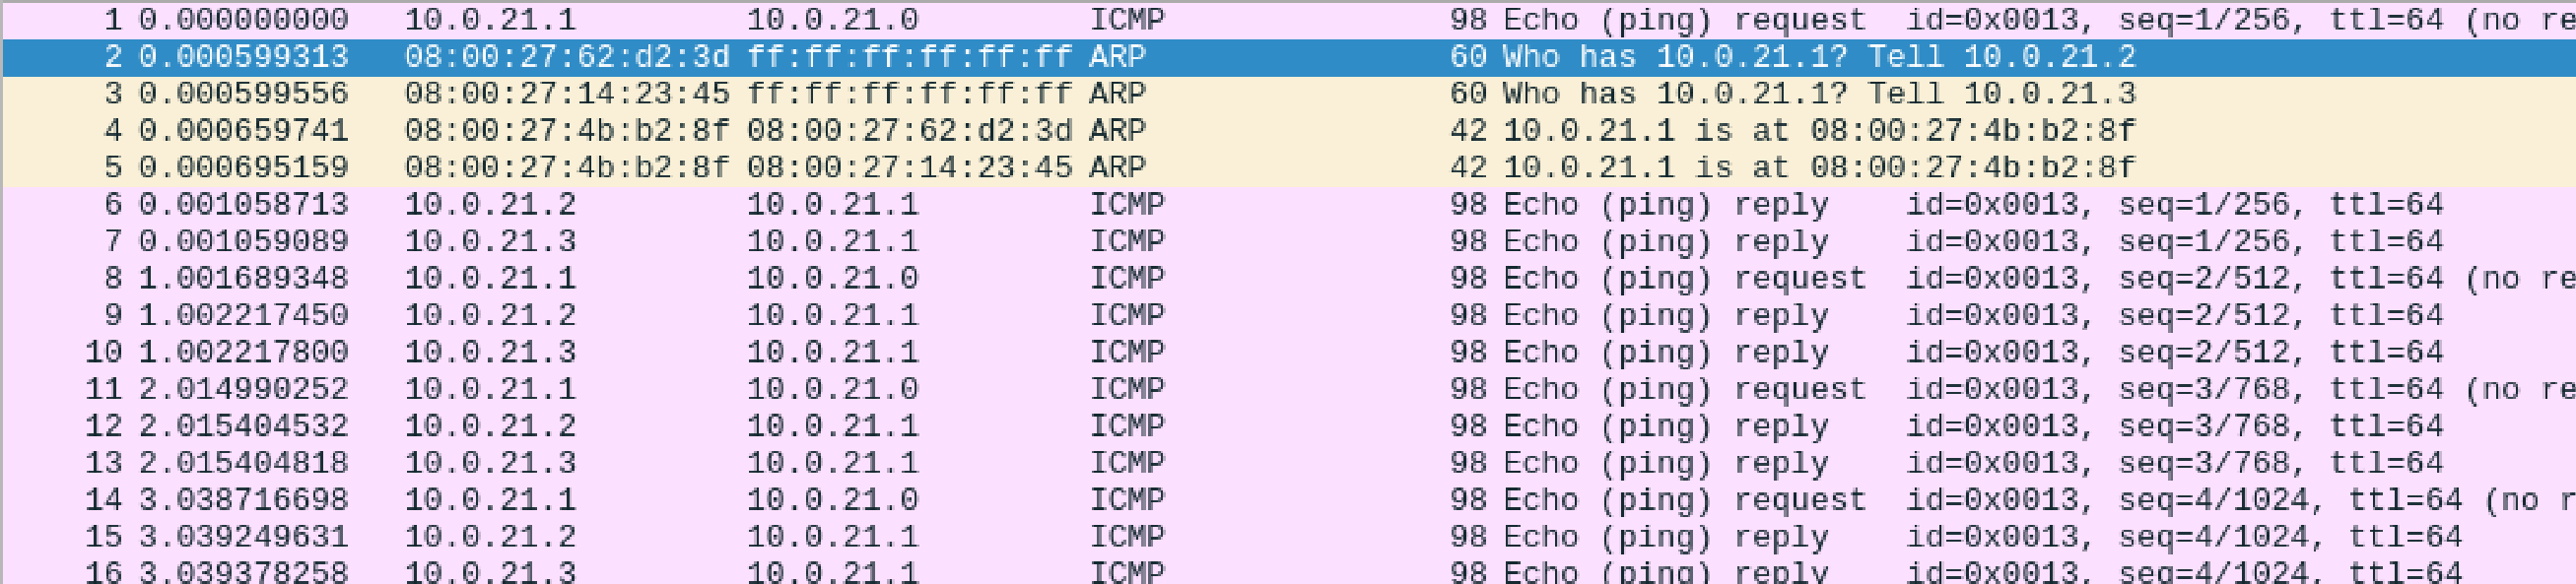
\includegraphics[width=0.7\textwidth]{indirizzorete.png}
\end{wrapfigure}

Si può notare come il comportamento quando si esegue il ping verso l’indirizzo di rete sia identico a quello analizzato quando si esegue il ping all’indirizzo broadcast.

\section{Indirizzi duplicati}

Abbiamo configurato la rete in modo che l’indirizzo ip degli host H1 e H3 sia uguale a 10.0.21.1/27

\subsection{Ping da H2 a H1}

%\hspace{1cm}
\begin{wrapfigure}{r}{0.66\textwidth} %this figure will be at the right
 \vspace{-10pt}
    \centering
    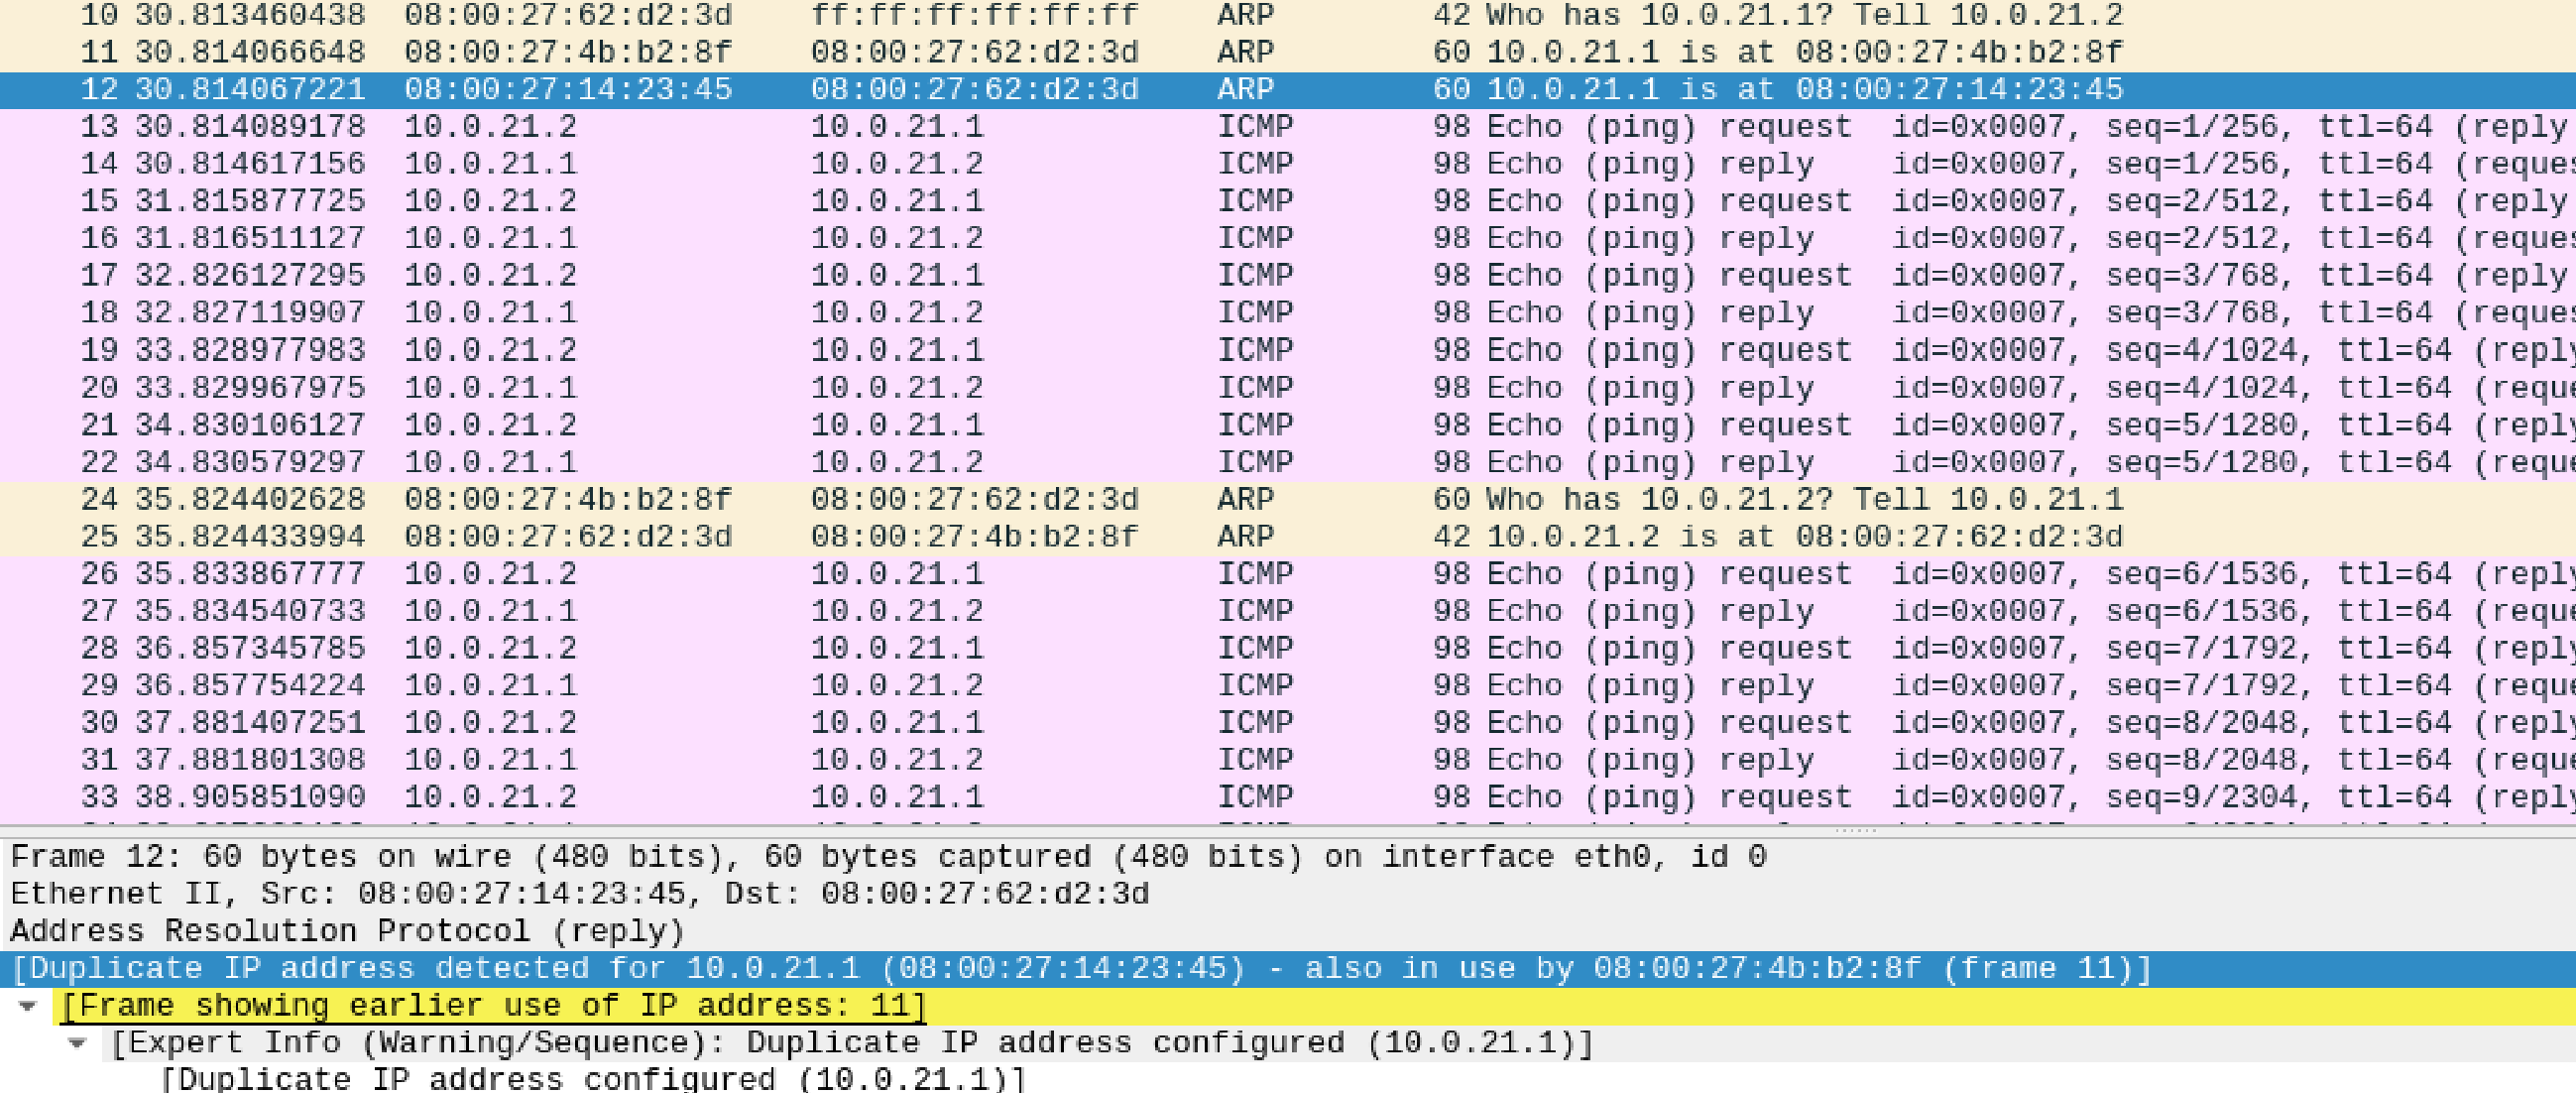
\includegraphics[width=0.6\textwidth]{duplicati1.png}
    \vspace{-5pt}
    \caption{elenco pacchetti in transito su H1}
   
% \end{wrapfigure}
\rule[5mm]{10cm}{0.5pt}
%\rule[5mm]{0mm}{0.5cm}
%\rule{8cm}{0.8pt}
% \begin{wrapfigure}{r}{0.66\textwidth} %this figure will be at the right
  \centering
  \vspace{-5pt}
  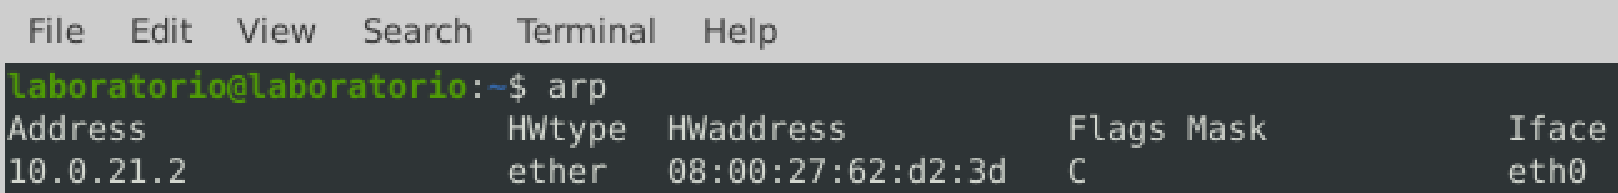
\includegraphics[width=0.6\textwidth]{host1ARP.png}
  \vspace{-4pt}
  \caption{host1}
  \vspace{-20pt}
\end{wrapfigure}
% \begin{figure}
%     \begin{minipage}{0.67\textwidth}
%       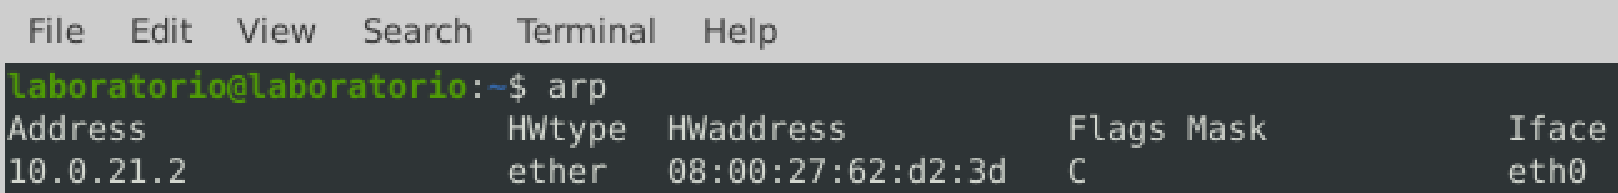
\includegraphics[width=\textwidth]{host1ARP.png}
%     \end{minipage}\hfill
%     \begin{minipage}{0.3\textwidth}
%       \caption{
%          host 1
%       } \label{fig:03-03}
%     \end{minipage}
%   \end{figure}

Se eseguo il ping da H2 verso l’ip 10.0.21.1, wireshark catturerà l’ARP request di H2 e le due ARP reply da parte di H3 e H1. ARP considera solo la prima risposta e marcherà la seconda come \textit{duplicate ip address}, quindi il primo tra H3 e H1 riceverà due \textit{ARP Reply}, mentre il secondo non riceverà nulla.
Come si può notare il rinfresco delle tabelle ARP non viene eseguito tramite un messaggio broadcast, ma viene usato l’indirizzo MAC già presente precedentemente nell'ARP Table. Ad esempio nel nostro caso, la comunicazione avviene solo tra H2 e H1.


\vspace{2cm}
\subsection{Ping da H1 e H3 a H2}



%\hspace{1.2cm}
\begin{wrapfigure}{r}{0.75\textwidth} %this figure will be at the right
  \vspace{-10pt}
    \centering
      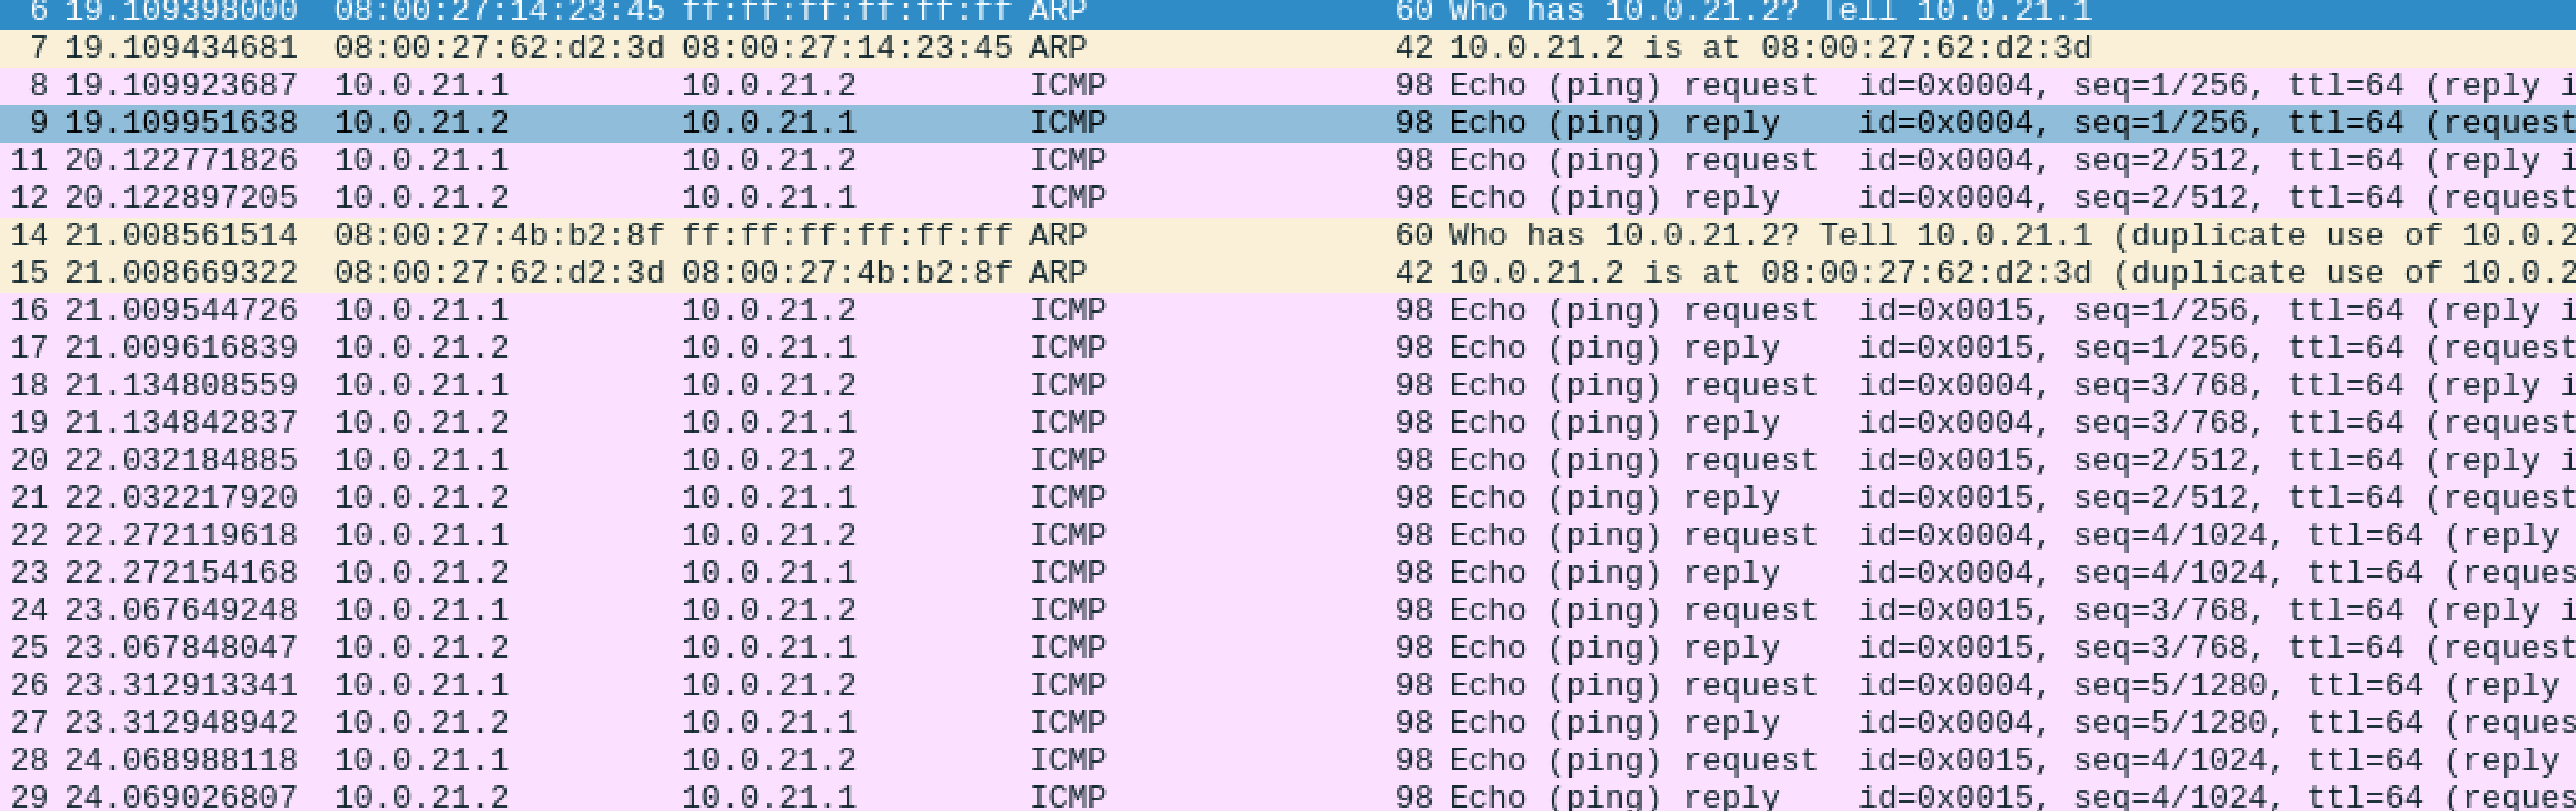
\includegraphics[width=0.75\textwidth]{es2.2host2.png}
      %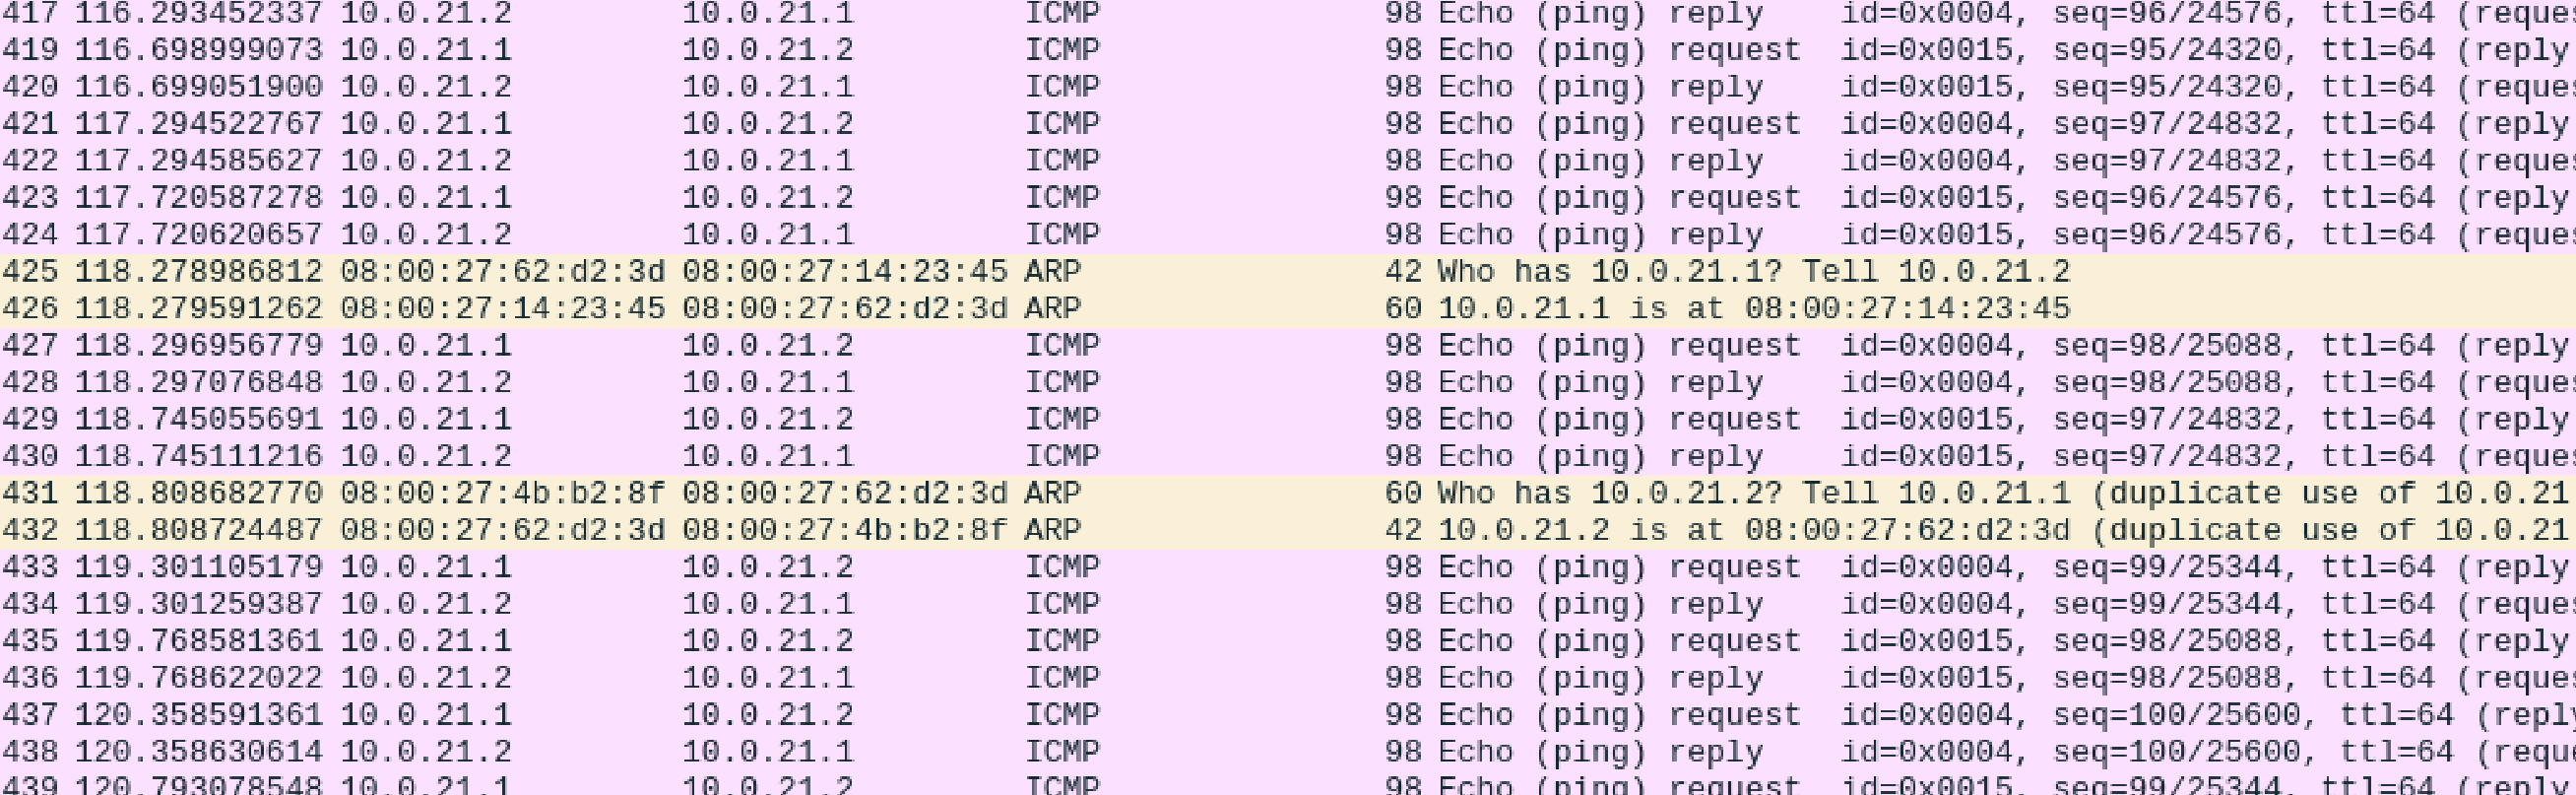
\includegraphics[width=0.75\textwidth]{Commutazione.png}
\end{wrapfigure}
Se invece eseguiamo il Ping contemporaneamente da H1 e H3 a H2, si può notare che H2 risponde in modo casuale e alternato ad entrambi.
Analizzando con wireshark il traffico in H2, notiamo all’inizio due ARP Request broadcast ad H2 a cui H2 risponda ad entrambe aggiornando conseguentemente la propria tabella alla richiesta più recente.
\pagebreak
 \begin{wrapfigure}{r}{0.75\textwidth} %this figure will be at the right
  \centering
    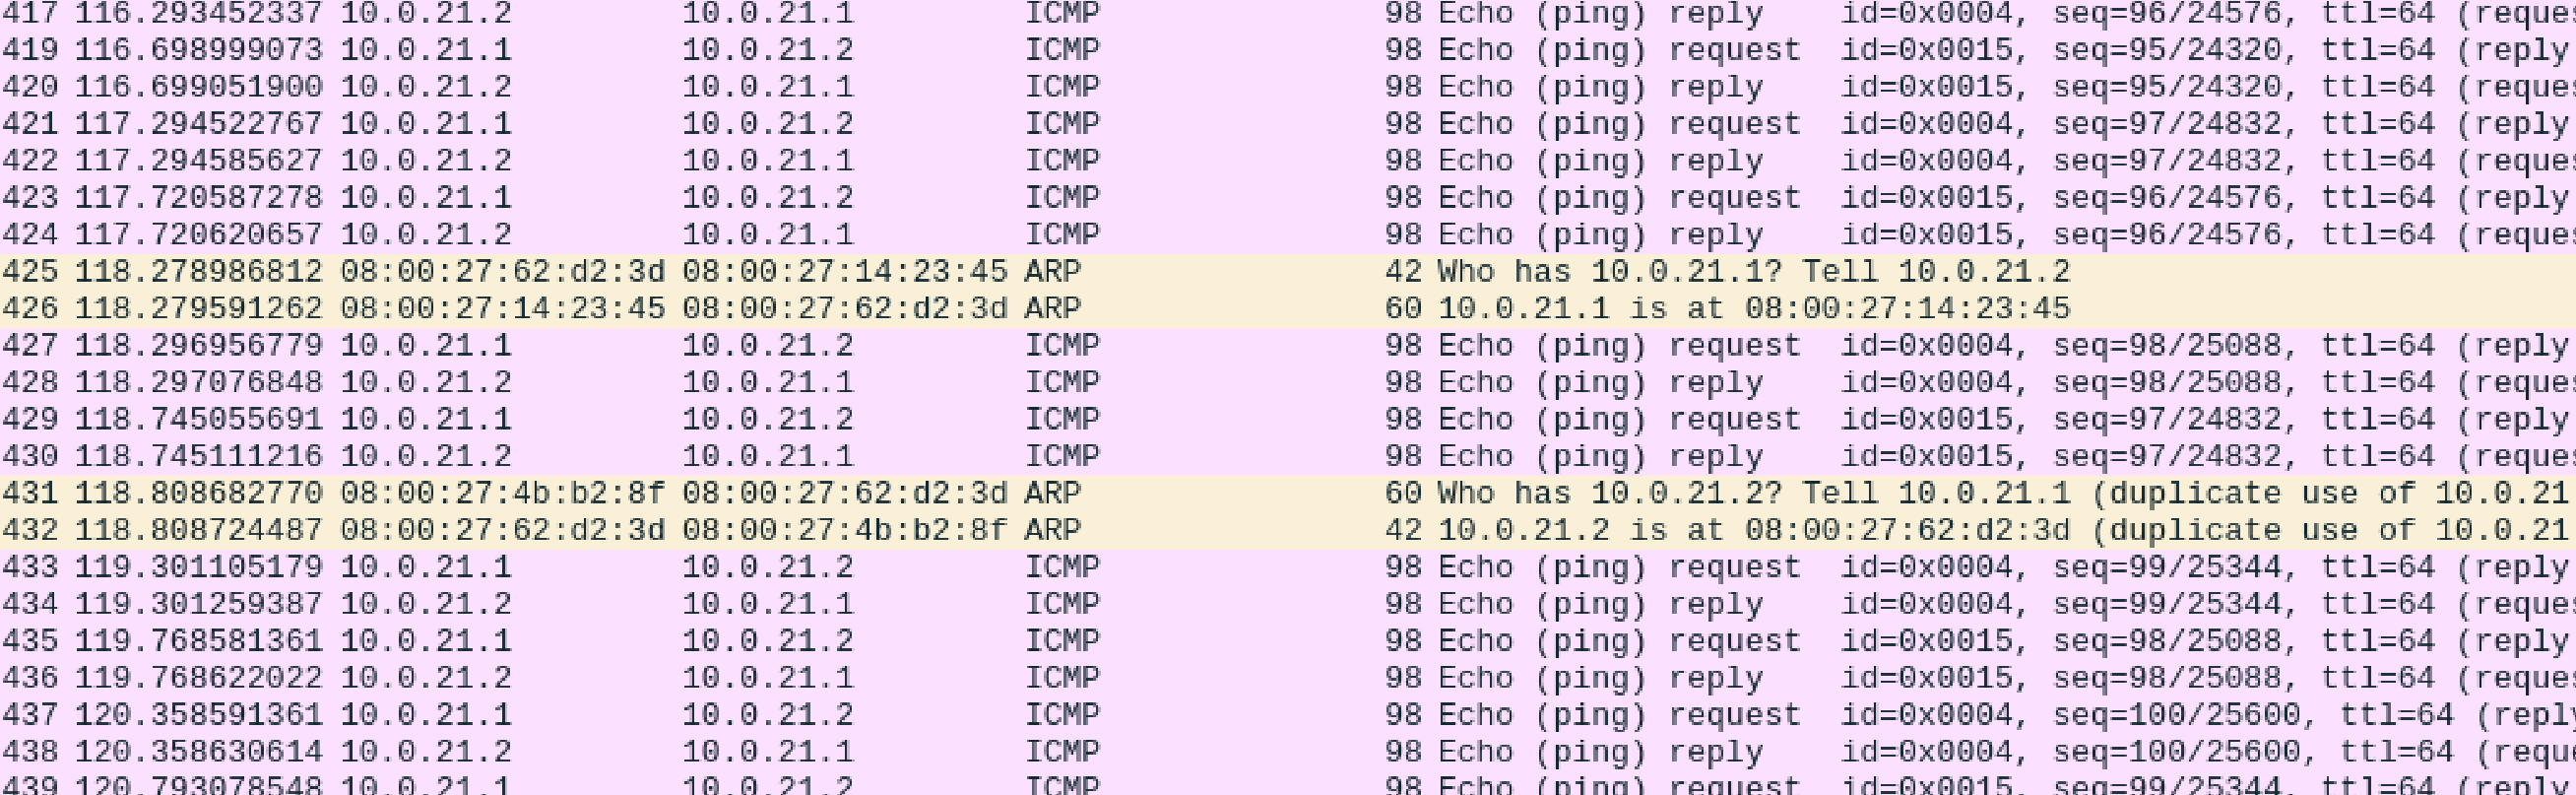
\includegraphics[width=0.75\textwidth]{Commutazione.png}
\end{wrapfigure}

H1 e H3 ad intervalli apparentemente casuali inviano con una richiesta unicast per rinfrescare la loro Arp Table ad H2 che di conseguenza aggiorna la propria tabella. Ad ogni aggiornamento, se è cambiata la tabella di ARP rispetto al momento precedente, si nota che cambiano anche le destinazioni delle Echo Reply, per questo motivo si nota l’alternanza di risposte tra H1 e H3.
I rinfreschi richiesti da H2 non modificheranno la tabella ARP, appunto perché la richiesta viene fatta in unicast.
Se analizziamo le catture sugli Host H1 e H3, si noterà che per ogni request ci saranno due reply, poiché ad H2 sono arrivate due richieste a cui rispondere. Se si riuscisse ha far partire il ping in modo contemporaneo si potrebbe apprezzare che le seconde Reply vengano definite come duplicate, ma si noterebbe anche che l’identificativo tra i due pacchetti ricevuti è diverso e solo uno corrisponde a quello dell’Host che sta effettivamente ricevendo.

Quindi le ARP table nella configurazione finale per H1 e H3 presentano l'entry che identifica H2, mentre quella di H2 conterrà il Mac dell’ultimo Host che ha fatto richiesta.

\section{Netmask sbagliate}
\begin{figure}[!htb]
    \begin{minipage}{0.48\textwidth}
        Abbiamo configurato la rete in modo che H1 veda all’interno della sua rete H2, ma H2 non veda H1 come un host appartenente alla propria sottorete.
    \end{minipage}\hfill
    \begin{minipage}{0.48\textwidth}
        \centering
        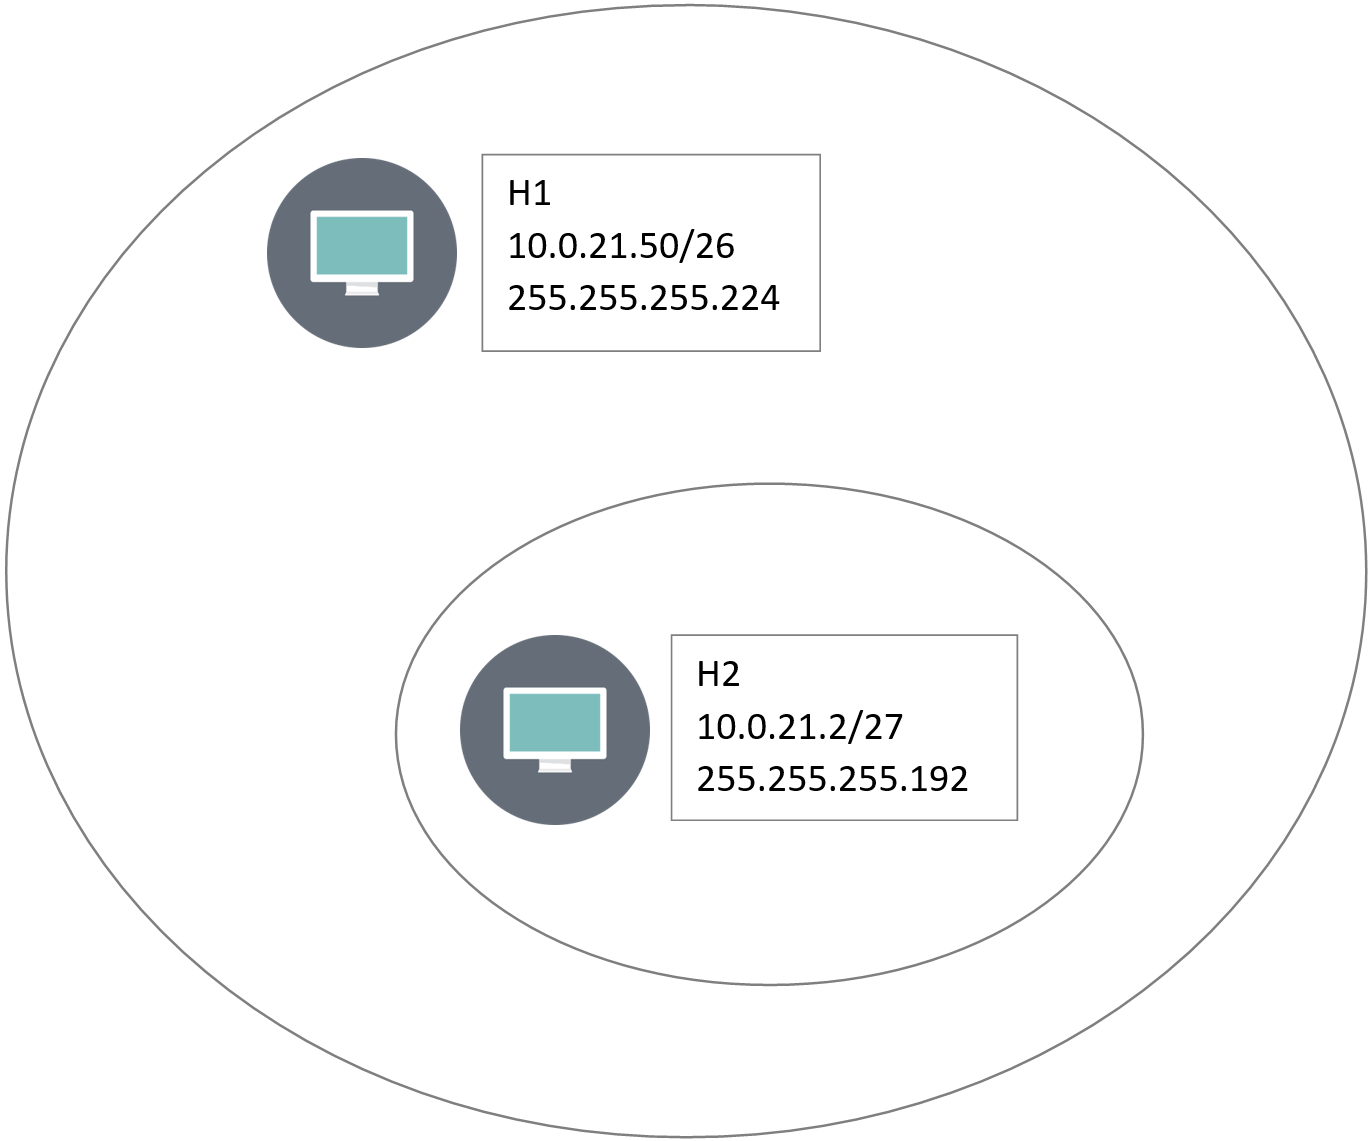
\includegraphics[width=0.7\linewidth]{es3.png}
    \end{minipage}
 \end{figure}


\subsection{Ping di H1 a H2}
\begin{figure}[!htb]
    \begin{minipage}{0.5\textwidth}
      Dal risultato si denota come H1 non riceva risposta da H2, poiché H1 manda inizialmente una ARP Request ad H2, ma H2 non potendo contattare un Host che non si trova all’interno della propria sottorete non invia nessuna \textit{ARP Reply}.
      \\La tabella ARP di H1 risulterà incompleta mentre quella di H2 risulterà vuota.
    \end{minipage}\hfill
    \begin{minipage}{0.5\textwidth}
      %\centering
      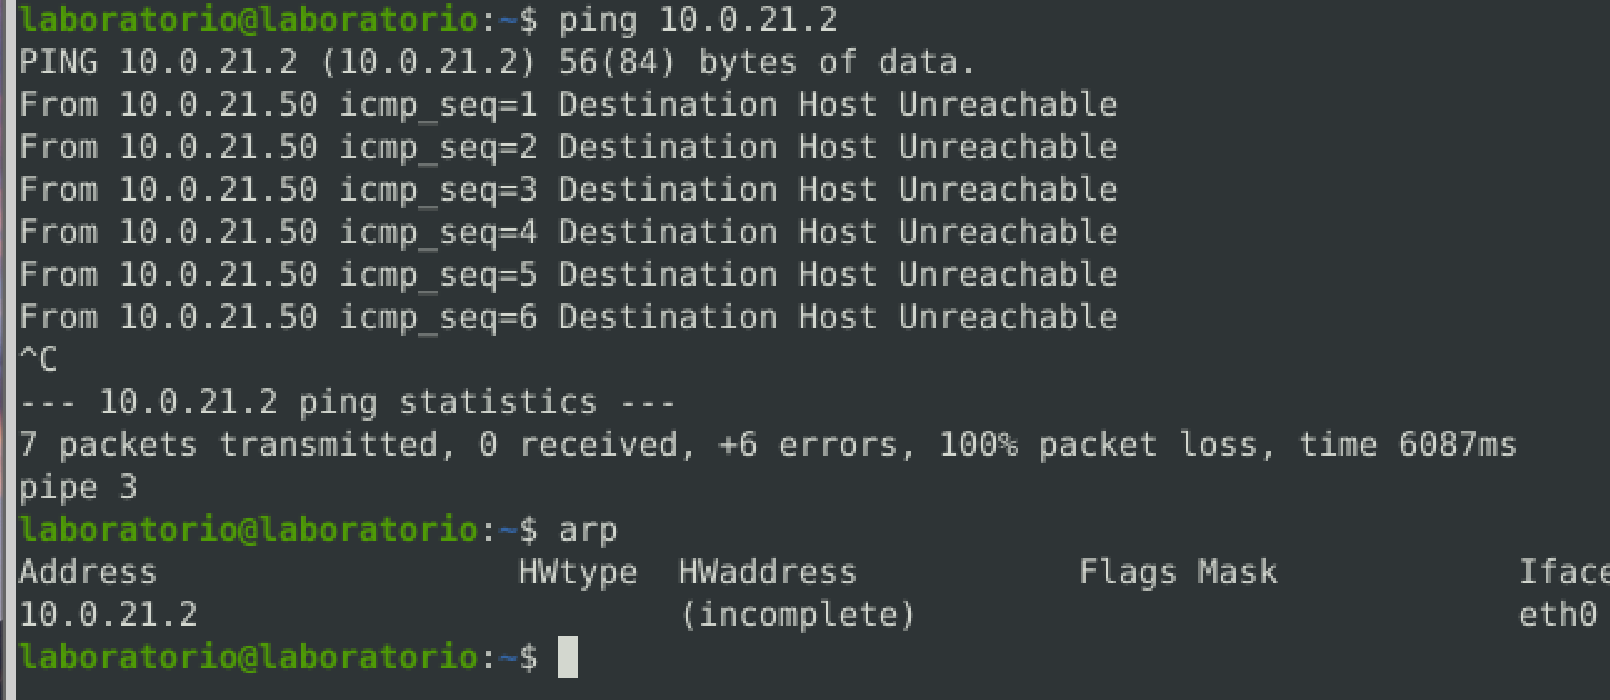
\includegraphics[width=0.8\linewidth,right]{es3hostUnreach.png}
    \end{minipage}
 \end{figure}


\subsection{Ping di H2 a H1}
\begin{figure}[!htb]
    \begin{minipage}{0.55\textwidth}
      H2 non può inviare nessuna ARP Request verso H1, e non essendo impostato nessun default gateway non può raggiungere nessun host esterno alla rete.
      Entrambe le ARP Table risulteranno quindi vuote.
    \end{minipage}\hfill
    \begin{minipage}{0.4\textwidth}
      \centering
      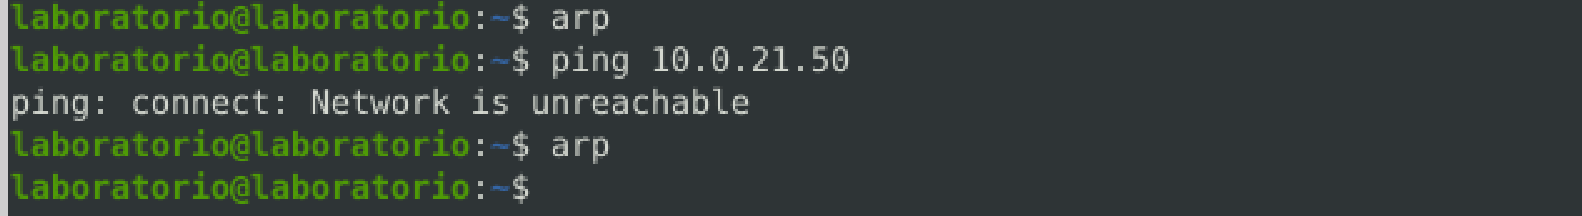
\includegraphics[width=1\linewidth]{es3NetworkUnreach.png}
    \end{minipage}
 \end{figure}
 \pagebreak
\section{Netmask sbagliate e broadcast in conflitto}
\begin{figure}[!htb]
    \begin{minipage}{0.48\textwidth}
    Abbiamo configurato la rete in modo che H1 veda all’interno della propria rete H2, ma H1 è l’indirizzo broadcast della sottorete di H2.
    \end{minipage}\hfill
    \begin{minipage}{0.48\textwidth}
      \centering
      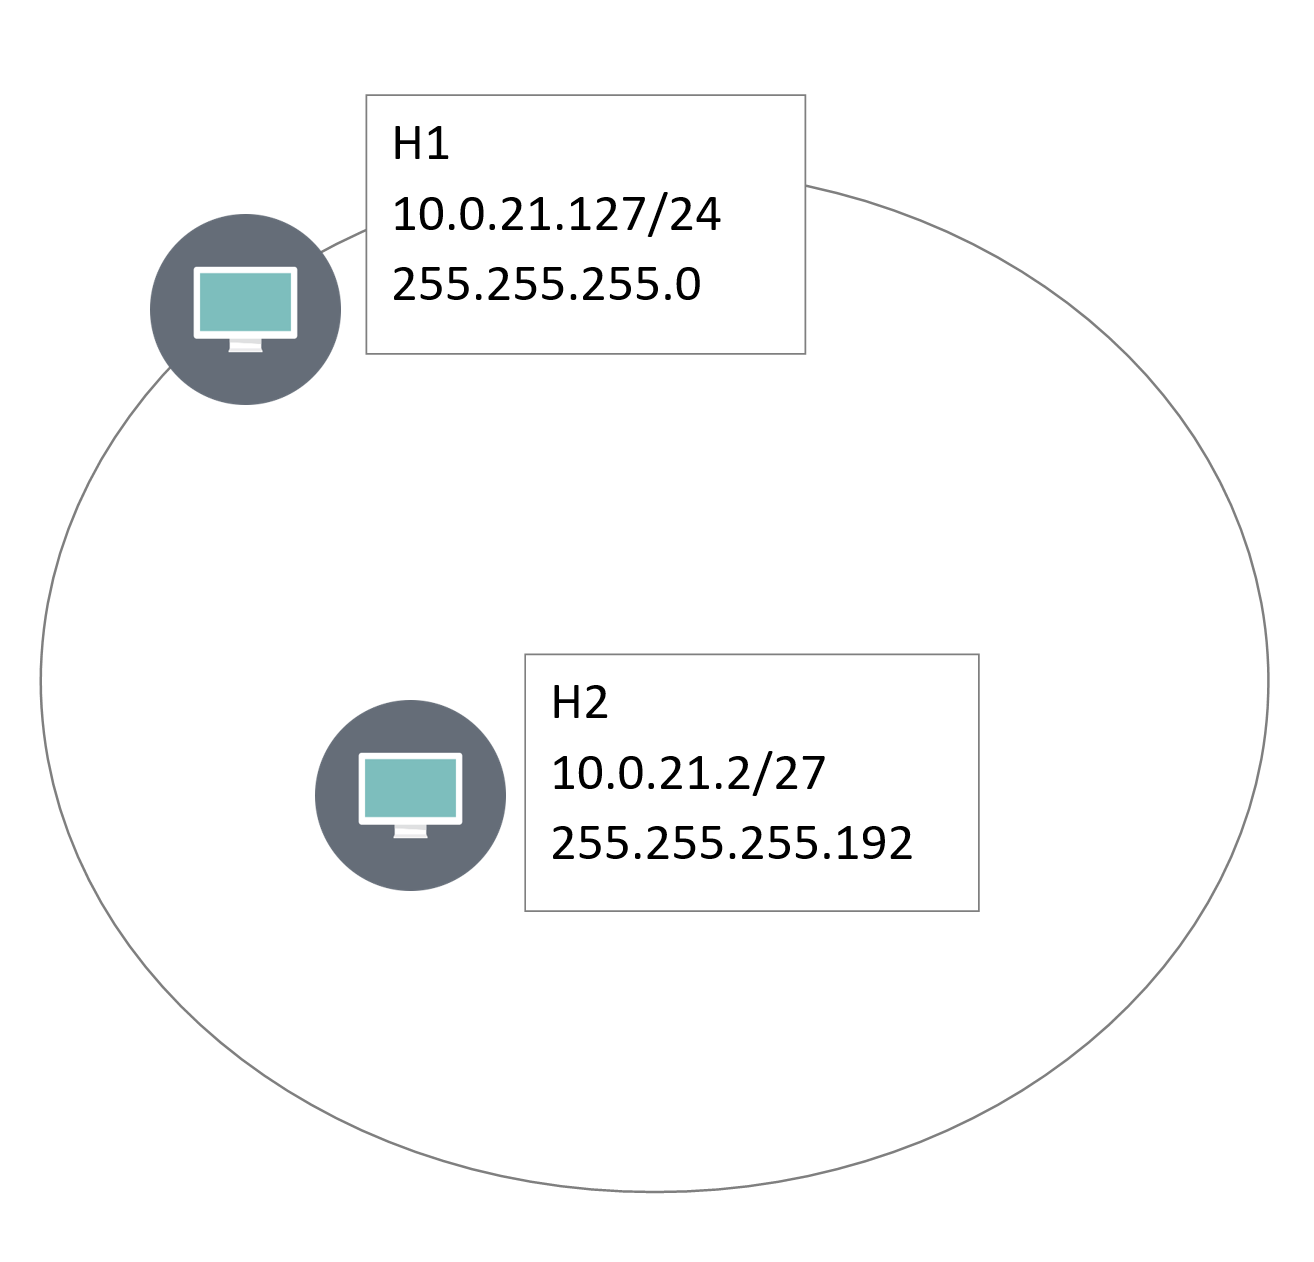
\includegraphics[width=0.7\linewidth]{es4.png}
    \end{minipage}
 \end{figure}

 \subsection{Ping di H1 a H2}

 \begin{figure}[!htb]
    \begin{minipage}{0.2\textwidth}
        In questo caso si è violata la semantica per la \textit{ARP Request} poiché l’indirizzo di \textit{Source} è quello di broadcast della sottorete di H2,quindi H2 non può rispondere alla richiesta.
        Le tabelle di ARP H1 sarà incompleta e quella di H2 sarà vuota.  
    \end{minipage}\hfill
    \begin{minipage}{0.78\textwidth}
      \centering
      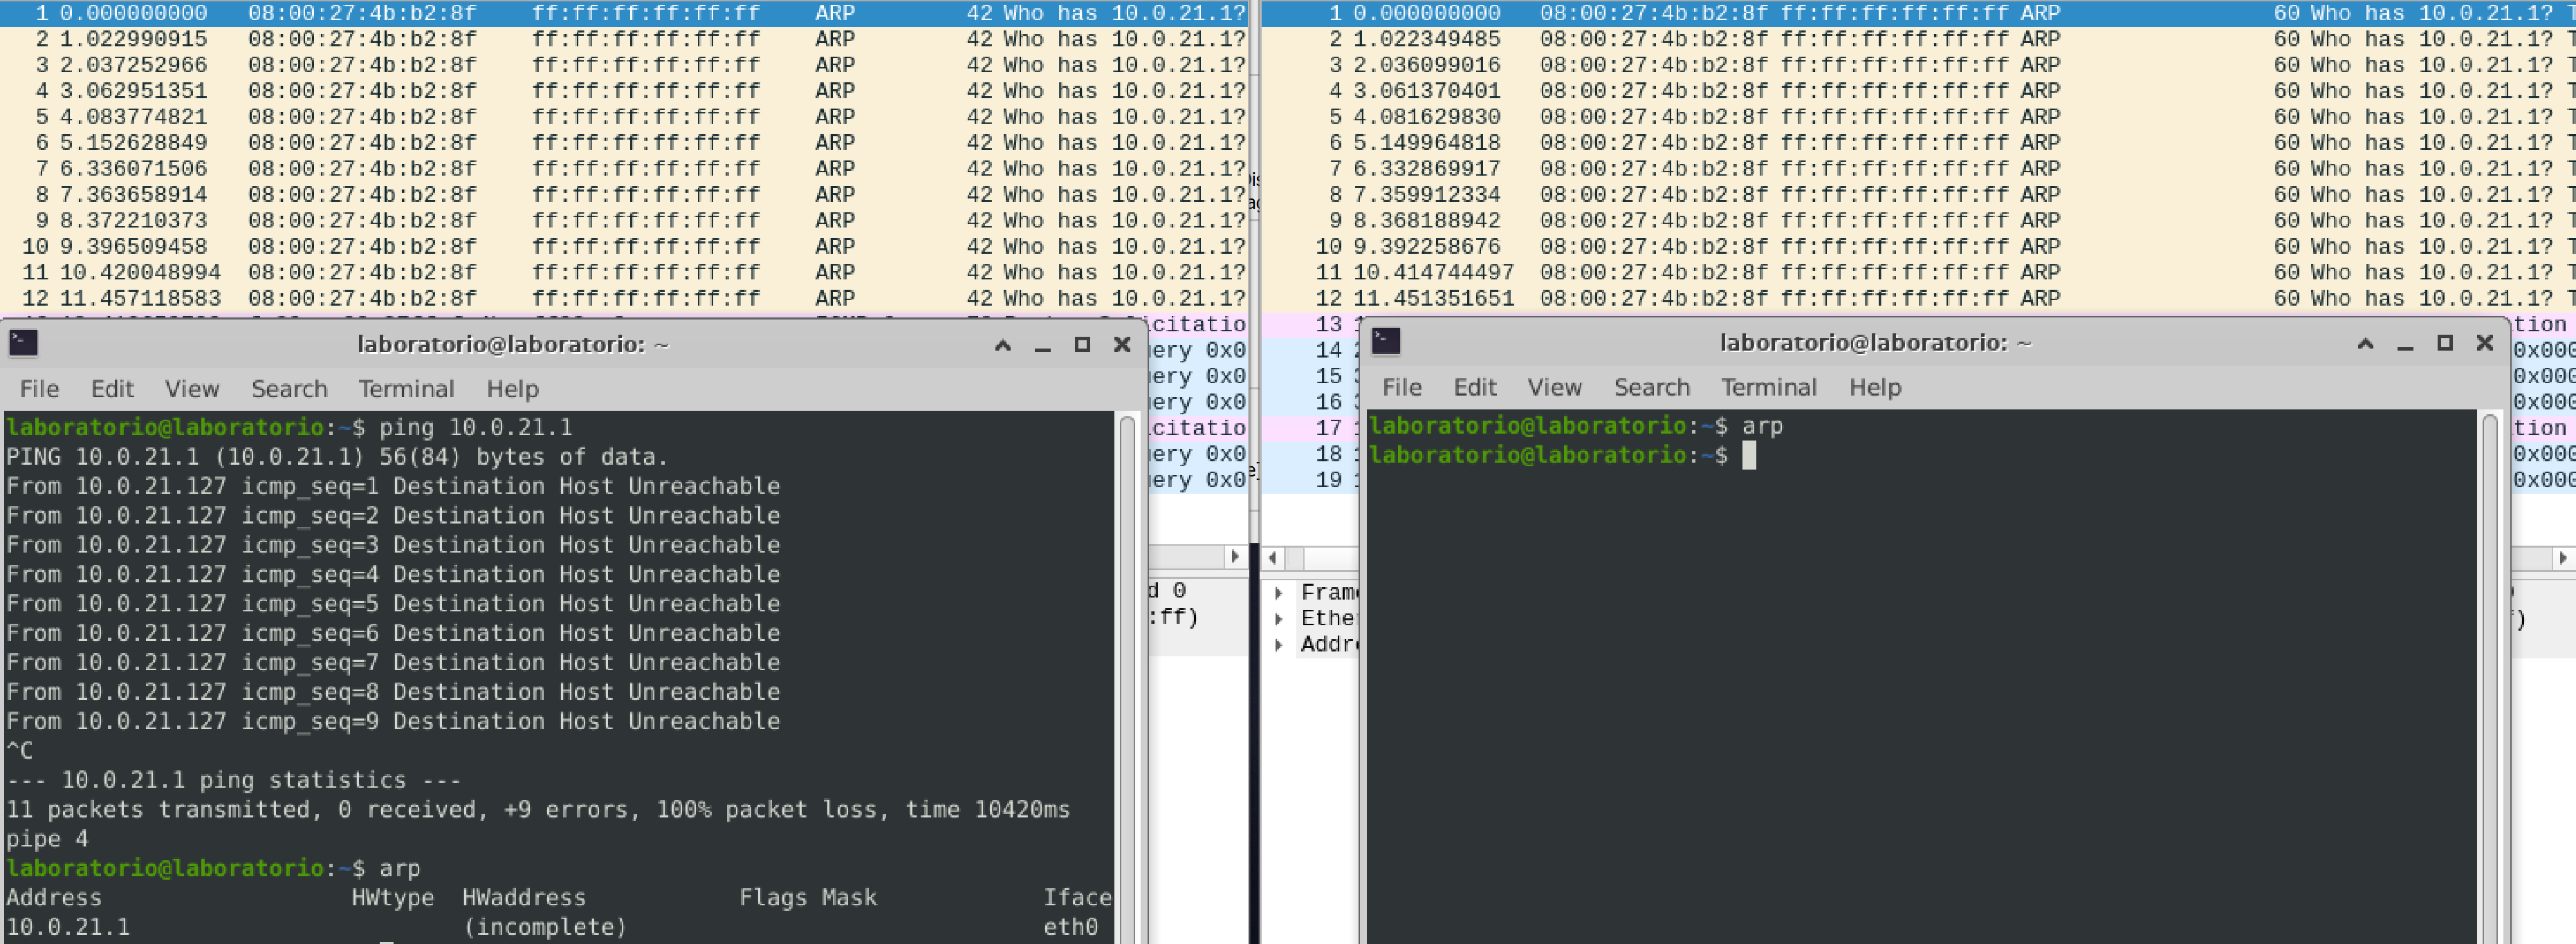
\includegraphics[width=1.05\linewidth]{es4.1.png}
    \end{minipage}
 \end{figure}

 \subsection{Ping di H2 a H1}

 Per effettuare questo ping bisogna utilizzare l’opzione -b per abilitare il ping al broadcast.
Le uniche risposte che riceverà sono quelle relative all’interfaccia di loopback, mentre non riceverà risposte da H1 perché per lo stesso motivo del punto precedente si sta violando la semantica della \textit{ARP Request}: H1 è sempre l’indirizzo di broadcast della sottorete di H2.
Le ARP Table quindi risultano uguali al punto precedente perché H2 non risponderà alla ARP Request di H1.


 \begin{figure}[!htb]
    \begin{minipage}{0.49\textwidth}
      \centering
      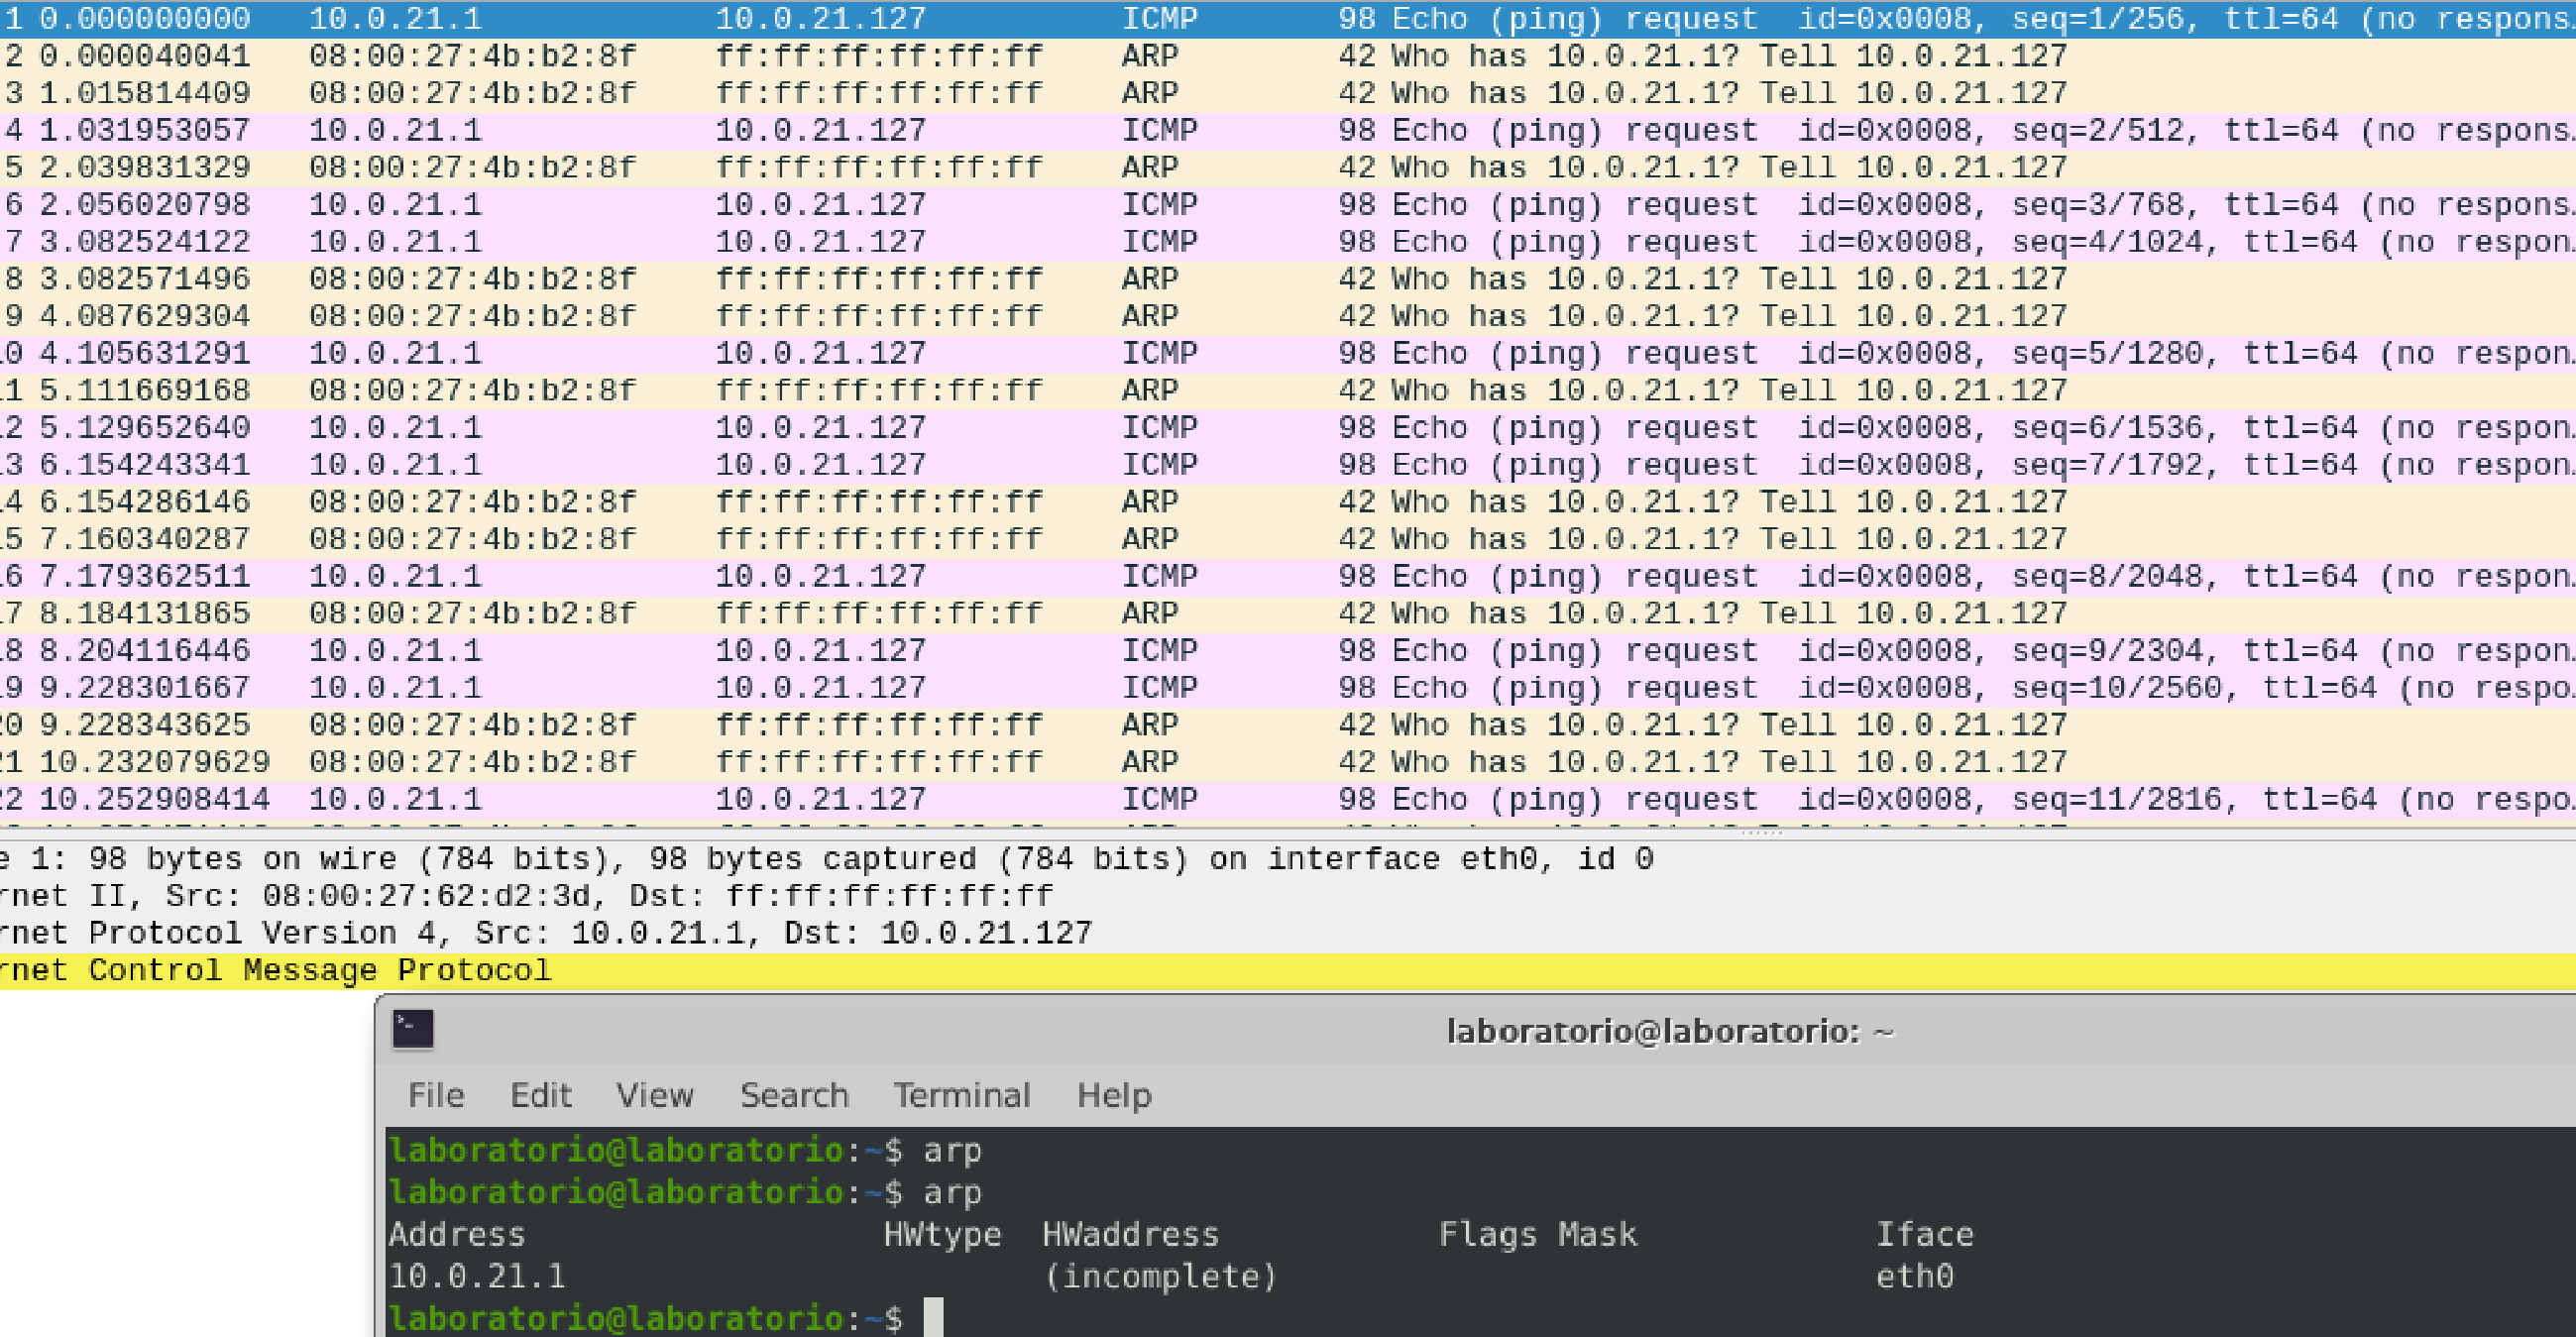
\includegraphics[width=1\linewidth]{es4.2.1.png}
    \end{minipage}\hfill
    \begin{minipage}{0.49\textwidth}
      \centering
      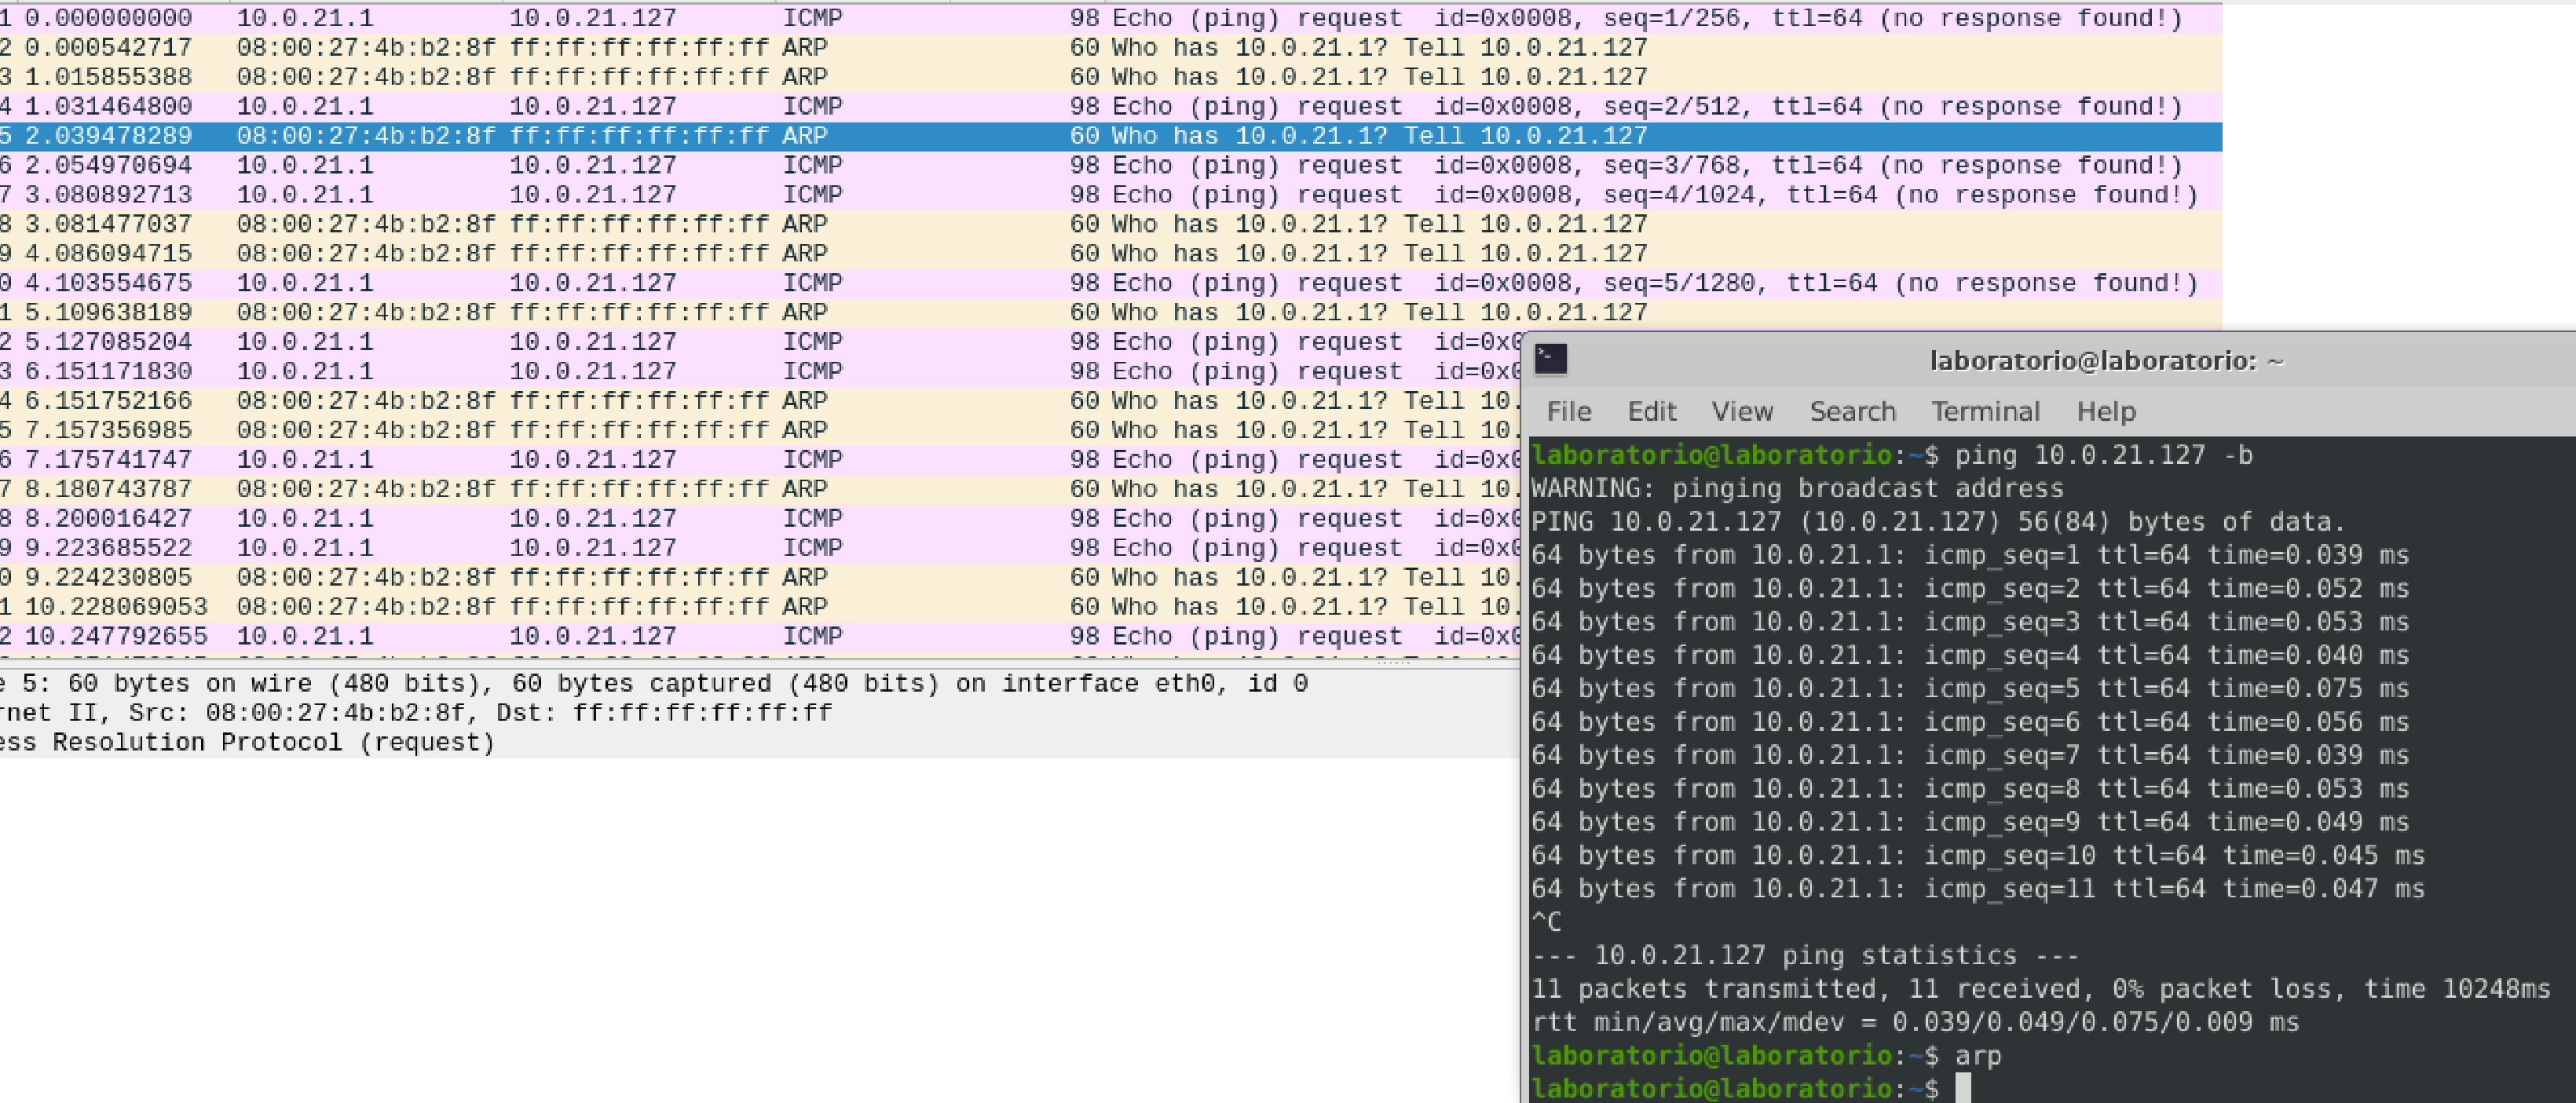
\includegraphics[width=1\linewidth]{es4.2.2.png}
    \end{minipage}
 \end{figure}
\end{document}